\chapter*{Progetto}
\addcontentsline{toc}{chapter}{Progetto} % add the chapter to the index
Ad affiancare questa relazione è stata realizzata una demo implementativa che è possibile provare navigando all'indirizzo \url{https://tendto.github.io/EW-showcase/}.
Al fine di visionare tutte le funzioni, è necessario dotarsi dell'estensione browser \href{https://metamask.io/}{MetaMask}, \href{https://energyweb.atlassian.net/wiki/spaces/EWF/pages/703201459/Volta+Connecting+to+Remote+RPC+and+Metamask}{connettersi alla rete Volta} e avere a disposizione qualche \href{https://voltafaucet.energyweb.org/}{Volta token}. \\

La \gls{dapp} (\autoref{lab:project}) rappresenta la sintesi del progetto, e ha come scopo quello di mostrare in azione le funzionalità \gls{ewns} (\autoref{sec:ewns}), \gls{did} (\autoref{sec:did}) e \gls{iam} (\autoref{sec:iam}), utilizzando, ove possibile, le librerie e i frameworks messi a disposizione da \gls{ew}.

\begin{figure}[h]
    \centering
    \subfloat[\centering \gls{did}]{{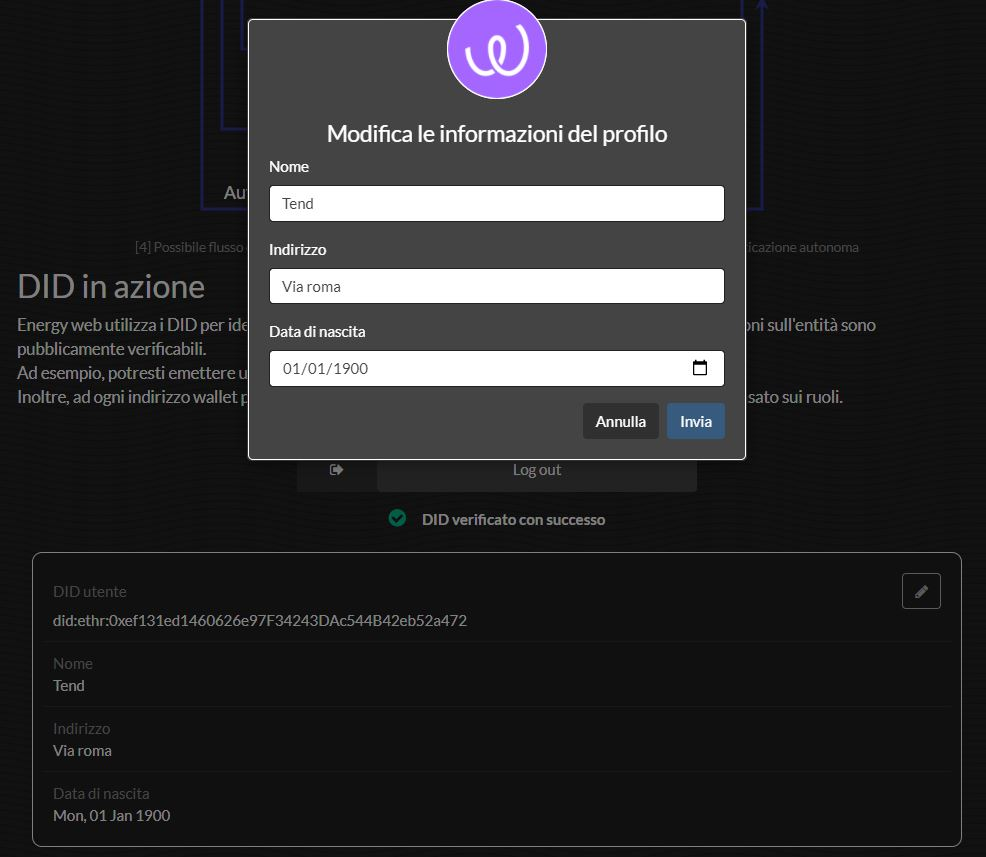
\includegraphics[width=6cm]{DID.jpg} }}
    \qquad
    \subfloat[\centering \gls{iam}]{{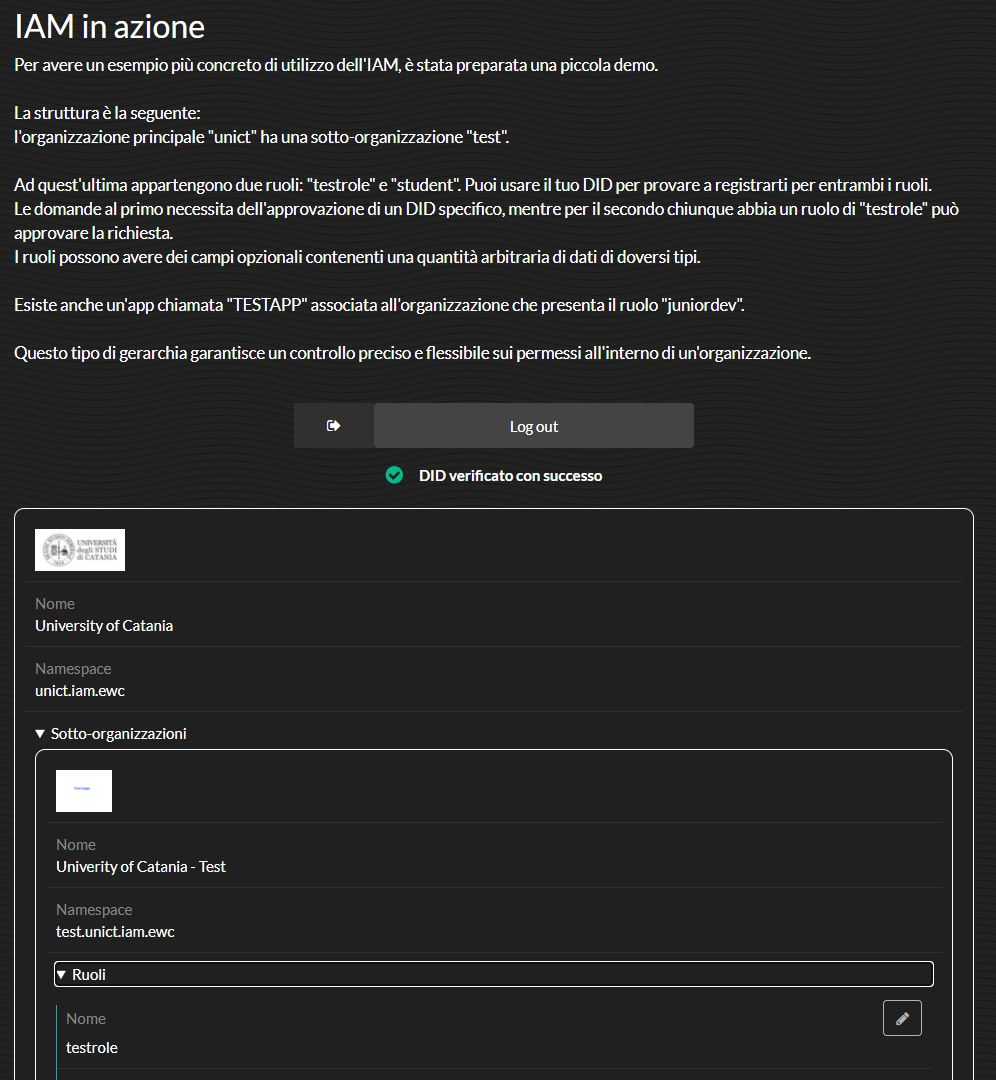
\includegraphics[width=6cm]{IAM.jpg} }}
    \caption{Screenshots della \gls{dapp}}
    \label{lab:project}
\end{figure}

\begin{figure}[h]
    \centering
    \subfloat[\centering Proprietario]{{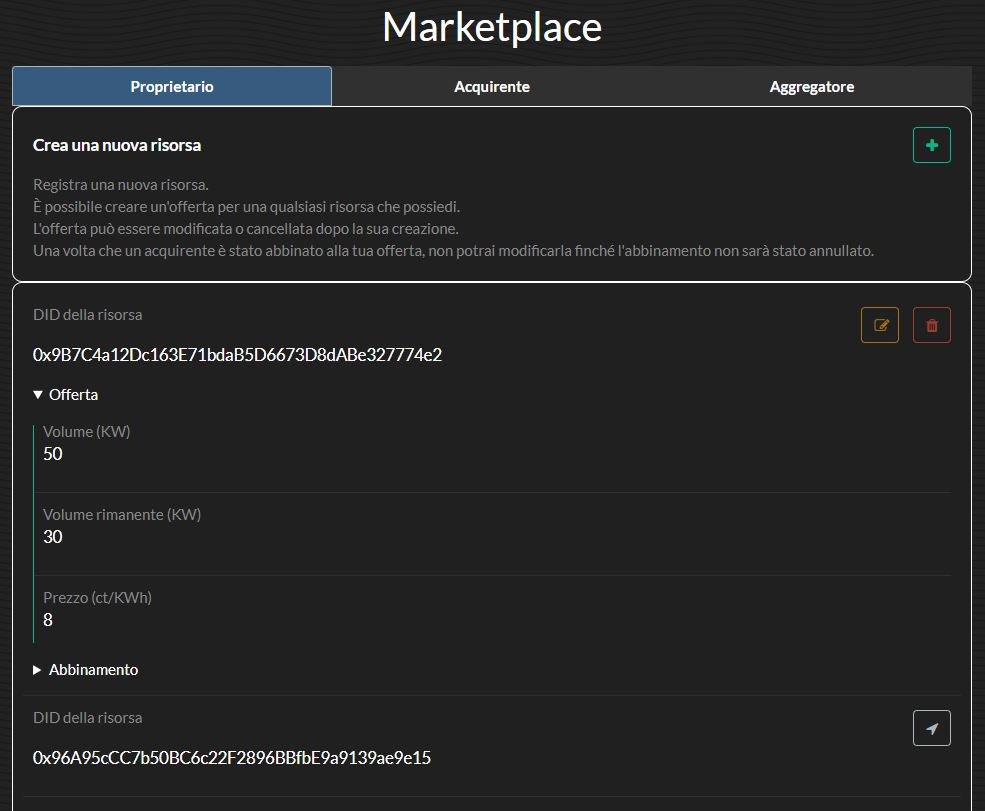
\includegraphics[width=6cm]{Marketplace1.jpg} }}
    \qquad
    \subfloat[\centering Aggregatore]{{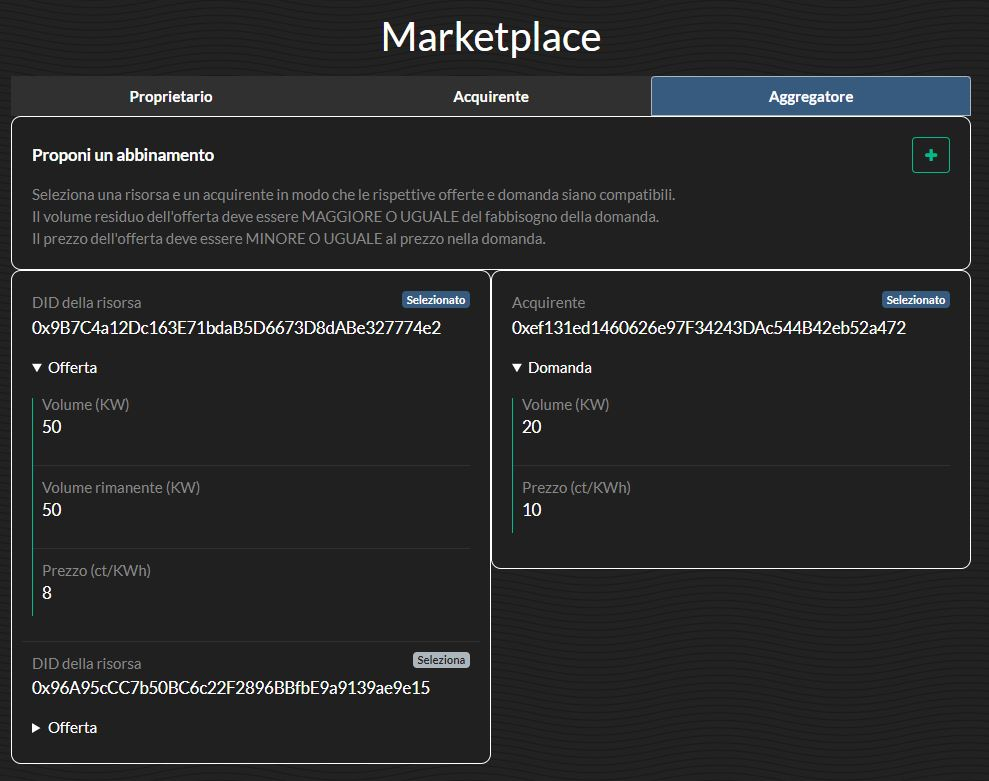
\includegraphics[width=6cm]{Marketplace2.jpg} }}
    \caption{Screenshots del Marketplace}
    \label{lab:marketplace}
\end{figure}

L'ultima sezione della \gls{dapp} comprende una implementazione molto semplificata di Energy Web Flex, chiamata Marketplace (\autoref{lab:marketplace}). \\

\newpage
Vengono individuati tre ruoli chiave: 
\begin{itemize}
    \item il proprietario di \gls{der} (\textbf{P}) - vende energia
    \item l'acquirente (\textbf{A}) - acquista energia
    \item l'aggregatore (\textbf{AGG}) - abbina domanda e offerta
\end{itemize}

Creare un abbinamento fra il primo e il secondo richiede generalmente il seguente procedimento:
\begin{enumerate}
    \item \textbf{P} propone un'offerta per i \gls{der} che possiede, specificando il volume di energia (kW) e il prezzo (ct/kWh). L'offerta può essere modificata o ritirata successivamente
    \item \textbf{A} pubblica una domanda con il volume di energia (kW) di cui ha bisogno e il prezzo massimo (ct/KWh) che è disposto a pagare. La domanda può essere modificata o ritirata successivamente
    \item AGG seleziona un'offerta e una domanda che formino una coppia valida e propone l'abbinamento. Da questo momento in poi offerta e domanda non possono più essere modificate fino a quando l'abbinamento proposto non viene accettato o rifiutato
    \item L'abbinamento proposto può essere accettato solo da \textbf{A}, ma può essere rifiutato sia da \textbf{P} che da \textbf{A}
    \item Una volta accettato, l'abbinamento entra in vigore.
    \item In qualsiasi momento sia \textbf{P} che \textbf{A} possono eliminare l'abbinamento
\end{enumerate}

Il Marketplace utilizza due smart contract presenti sulla Volta testnet:
\begin{itemize}
    \item \href{https://volta-explorer.energyweb.org/address/0x84d0c7284A869213CB047595d34d6044d9a7E14A/transactions}{Identity Manager (0x84d0c7284A869213CB047595d34d6044d9a7E14A)}, smart contract ufficiale sviluppato ed utilizzato da \gls{ew}
    \item \href{https://volta-explorer.energyweb.org/address/0x37dfeF9b9c56A81927Dfa73994E2fb23c3dd4b37/transactions}{Marketplace (0x37dfeF9b9c56A81927Dfa73994E2fb23c3dd4b37)}
\end{itemize}

L'intera documentazione e il codice dell'implementazione sono disponibili nella repository pubblica \href{https://github.com/TendTo/EW-showcase}{EW showcase} (\url{https://github.com/TendTo/EW-showcase}) su Github.